\documentclass{sig-alternate}

%!TEX root=../ast2016.tex

\usepackage{array}
\usepackage{multirow}
\usepackage{adjustbox}

%!TEX root=../ast2016.tex

% Important numbers
\newcommand{\numschemas}{30\xspace}

% Highlight outstanding issues
\newcommand{\todo}[1]{{\color{red}$<$TODO: #1$>$}}
\newcommand{\query}[1]{{\color{blue}$<$QUERY: #1$>$}}
\newcommand{\answer}[1]{{\color{ForestGreen}$<$ANSWER: #1$>$}}
\newcommand{\thesis}[1]{{\color{Plum}$<$THESIS PROSE: #1$>$}}
\newcommand{\paper}[2]{{\color{Orange}$<$#1: #2$>$}}

% Definition-type environments
\newtheorem{definition}{Definition}
\newtheorem{criterion}{Criterion}

% Extra heading levels
\newcommand{\inlineheading}[1]{\vspace{1ex}{\noindent}{\bf #1.}~}
\newcommand{\secondaryinlineheading}[1]{\vspace{1ex}{\noindent}{\it #1.}~}

% Code style macros
\newcommand{\sql}[1]{{\normalfont{\texttt{#1}}}} % added \normalfont, so that SQL is not italicized inside definitions
\newcommand{\smsql}[1]{{\scriptsize{\sql{#1}}}}
\newcommand{\quot}[1]{\textquotesingle #1\textquotesingle}
\newcommand{\sqlquot}[1]{\sql{\quot{#1}}}

% Textual shortcuts
\newcommand{\sa}{{\it SchemaAnalyst}\xspace}
\newcommand{\SA}{\sa}
\newcommand{\SchemaAnalyst}{\sa}
\newcommand{\schemaanalyst}{\sa}
\newcommand{\sawebsite}{\url{http://www.schemaanalyst.org}}

\newcommand{\Original}{Original\xspace}
\newcommand{\VirtualMutationAnalysis}{Virtual Mutation Analysis\xspace}
\newcommand{\VMA}{\VirtualMutationAnalysis}

\newcommand{\NistWeather}{NistWeather\xspace}
\newcommand{\NW}{\NistWeather}

\newcommand{\DBMonster}{{\it DBMonster}\xspace}
\newcommand{\avm}{{\it AVM}\xspace}
\newcommand{\AVM}{\avm}
\newcommand{\theAVM}{the \avm}
\newcommand{\TheAVM}{The \avm}
\newcommand{\rand}{{\it Random$^{+}$}\xspace}
\newcommand{\random}{\rand}
\newcommand{\Random}{\rand}
\newcommand{\rnd}{\rand}

\newcommand{\postgres}{PostgreSQL\xspace}
\newcommand{\postgresql}{\postgres}
\newcommand{\Postgres}{\postgres}
\newcommand{\PostgreSQL}{\postgres}
\newcommand{\hypersql}{HyperSQL\xspace}
\newcommand{\hsqldb}{\hypersql}
\newcommand{\HSQLDB}{\hypersql}
\newcommand{\HyperSQL}{\hypersql}
\newcommand{\postgreshypersql}{\postgres/\hypersql}
\newcommand{\sqlite}{SQLite\xspace}
\newcommand{\SQLite}{\sqlite}

\newcommand{\CHECK}{\sql{CHECK}\xspace}
\newcommand{\CHECKs}{\sql{CHECK}s\xspace}
\newcommand{\CC}{\CHECK constraint\xspace}
\newcommand{\CCs}{\CHECK constraints\xspace}

\newcommand{\fk}{foreign key\xspace}
\newcommand{\fks}{foreign keys\xspace}
\newcommand{\FK}{\sql{FOREIGN KEY}\xspace}
\newcommand{\FKs}{\sql{FOREIGN KEY}s\xspace}
\newcommand{\FKC}{\FK constraint\xspace}
\newcommand{\FKCs}{\FK constraints\xspace}

\newcommand{\NOTNULL}{\sql{NOT NULL}\xspace}
\newcommand{\NOTNULLs}{\sql{NOT NULL}s\xspace}
\newcommand{\NNC}{\sql{NOT NULL} constraint\xspace}
\newcommand{\NNCs}{\sql{NOT NULL} constraints\xspace}

\newcommand{\pk}{primary key\xspace}
\newcommand{\pks}{primary keys\xspace}
\newcommand{\PK}{\sql{PRIMARY KEY}\xspace}
\newcommand{\PKs}{\sql{PRIMARY KEY}s\xspace}
\newcommand{\PKC}{\PK constraint\xspace}
\newcommand{\PKCs}{\PK constraints\xspace}

\newcommand{\UNIQUE}{\sql{UNIQUE}\xspace}
\newcommand{\UC}{\UNIQUE constraint\xspace}
\newcommand{\UNIQUEs}{\sql{UNIQUE}s\xspace}
\newcommand{\UCs}{\UNIQUE constraints\xspace}

\newcommand{\INSERT}{\sql{INSERT}\xspace}
\newcommand{\INSERTs}{\sql{INSERT}s\xspace}
\newcommand{\NULL}{\sql{NULL}\xspace}
\newcommand{\NULLs}{\sql{NULL}s\xspace}

\newcommand{\icp}{integrity constraint predicate\xspace}
\newcommand{\icps}{integrity constraint predicates\xspace}
\newcommand{\nc}{null condition\xspace}
\newcommand{\cc}{constraint condition\xspace}
\newcommand{\ccs}{constraint conditions\xspace}

\newcommand{\mannwhitney}{Mann--Whitney {\it U} test\xspace}
\newcommand{\wilcoxon}{Wilcoxon rank-sum test\xspace}
\newcommand{\pvalue}{{\it p}-value\xspace}
\newcommand{\bfpvalue}{\textbf{\textit{p}-value}\xspace}
\newcommand{\atwelve}{\^{A}\textsubscript{12}\xspace}
\newcommand{\bfatwelve}{\textbf{\textit{\^{A}}}$\mathbf{_{12}}$\xspace}

\newcommand{\etal}{et al.\xspace}

% Floats
\newcommand{\Figure}[1]{Figure~\ref{#1}\xspace}
\newcommand{\Section}[1]{Section~\ref{#1}\xspace}
\newcommand{\Table}[1]{Table~\ref{#1}\xspace}

%% To help ensure consistent float scaling
\def \algorithmfigurescalefactor {0.7}
\def \tablescalefactor {0.85}

%% Rotated table column type
\newcolumntype{R}[2]{%
    >{\adjustbox{minipage=6em,angle=#1,lap=\width-(#2)}\bgroup}%
    l%
    <{\egroup}%
}
\newcommand*\rot{\multicolumn{1}{R{60}{1.5em}}}

%% Highlight command for coloured highlight in listings
\newcommand{\reducedstrut}{\vrule width 0pt height \ht\strutbox depth \dp\strutbox\relax}
\newcommand{\highlight}[1]{%
  \begingroup
  \setlength{\fboxsep}{0pt}%
  \colorbox{red!20}{\reducedstrut#1\/}%
  \endgroup
}

% Equations
\newcommand{\eqnull}{= \relnull}
\newcommand{\existsinrel}[2]{\exists \inrel{#1}{#2}}
\newcommand{\forallinrel}[2]{\forall \inrel{#1}{#2}}
\newcommand{\inrel}[2]{#1 \in \: #2}
\newcommand{\neqnull}{\neq \relnull}
\newcommand{\relnull}{\bot}
\newcommand{\select}[2]{#1 (#2)}
\newcommand{\selecteqnull}[2]{\select{#1}{#2} \eqnull}
\newcommand{\selectneqnull}[2]{\select{#1}{#2} \neqnull}
\newcommand{\selectneq}[3]{\select{#1}{#3} \: \neq \: \select{#2}{#3}}
\newcommand{\selecteq}[3]{\select{#1}{#3} \: = \: \select{#2}{#3}}
\newcommand{\selecteqexp}[4]{\select{#1}{#3} \: = \: \select{#2}{#4}}
\newcommand{\smallwedge}{\: \wedge \:}
\newcommand{\smallvee}{\: \vee \:}

\let\oldemptyset\emptyset
\let\emptyset\varnothing

% Algorithms in figures
\newcommand{\tinybullet}{$\vcenter{\hbox{\tiny$\bullet$}} \;$}
\newcommand{\atab}{\hspace{3ex}}
\newcommand{\wheretab}{\hspace{2ex}}
\newcommand{\exptab}{\hspace{2.5ex}}
\newcommand{\smallvspace}{\vspace{0.5ex}}
\newcommand{\closeblock}{\vspace{1ex}}
\newcommand{\closemajorblock}{\vspace{2ex}}

% Comments
\newcommand{\rem}[1]{}

% RQs
\newcommand{\conclusion}[2]{\vspace{1mm} \noindent {\bf Conclusion for #1:} #2}


\begin{document}

% DOI
\doi{...}

% ISBN
\isbn{...}

%% Due to our small subjects we decided to drop this title:
% \title{Using Virtual Mutant Evaluation to Achieve Scalability in Relational Database Schema Mutation Analysis \vspace*{-.1in}}
% \title{Achieving Scalability in Relational Database Mutation Analysis Through Virtual Mutant Execution}
% \title{Achieving Scalability in Relational Database Schema Mutation Analysis Through Virtual Mutant Evaluation}

\title{Virtual Mutation Analysis of Relational Database Schemas  \vspace*{-.1in}}
% Virtual Analysis of Relational Schema Mutants
% Virtualised Analysis of Relational Schema Mutants?
% Virtualisation of Mutation Analysis for Relational Schema Mutants
% Virtual Analysis of Relational Database Schema Mutants - Too long!
% Virtual Mutation Analysis of Relational Schema Mutants - Mutation..Mutants

\numberofauthors{3}

\author{
\alignauthor
Chris J. Wright\\
\affaddr{University of Sheffield, UK}
\alignauthor
Phil McMinn\\
\affaddr{University of Sheffield, UK}
\alignauthor
Gregory M. Kapfhammer\\
\affaddr{Allegheny College, USA}}

\maketitle

%% PM: this seemed to be unbalancing the top of the columns
%\vspace*{-.75in}

%!TEX root=../ast2016.tex

\begin{abstract}
%% Chris's original bullet points:
%   \begin{itemize}
%       \item Relational schemas can include constraints that contain business logic so need to be tested.
%       \item Mutation analysis can be used to model faults of omission and commission in constraints.
%       \item As with mutation analysis elsewhere, it can be costly (regardless of prior researched optimisations).
%       \item Virtual analysis exploits an existing model of database behaviour, used elsewhere for data generation, to reduce this \todo{to/by substantial figure here}.
%       \item Therefore we can mutate even large schemas quickly, making it a practically feasible testing technique.
%   \end{itemize}

%% Why this topic is important
Relational databases are a vital component of many modern software applications.
%
%% What the schema is, introduce integrity constraints
Key to the definition of the database schema---which specifies what types of data will be stored in the database and the structure in which the data is to be organized---are integrity constraints.
%
%% What integrity constraints are, and why we need to test them
Integrity constraints are conditions that protect and preserve the consistency and validity of data in the database, preventing data values that violate their rules from being admitted into database tables. They encode logic about the application concerned, and like any other component of a software application, need to be properly tested.
%
%% Introduce mutation analysis
Mutation analysis is a technique that has been successfully applied to integrity constraint testing, seeding database schema faults of both omission and commission. Yet, as for traditional mutation analysis for program testing, it is costly to perform,
%% cut because we're not mentioning scalability now...
% and tends not to scale well where large numbers of mutant schemas are involved.
since every mutant schema needs to be evaluated against the test suite of concern to establish whether it exposes the fault.
%% The crux of our technique
One overhead incurred by database schema mutation is the cost of communicating with the database management system (DBMS). In this paper we seek to eliminate this cost by performing mutation analysis virtually on a local model of the DBMS, rather than on an actual, running instance that hosts the real database. We present an empirical evaluation of our virtual technique that shows that significantly improves the time taken to perform mutation analysis, improving the scalability of the technique.
%
%% Some stats
% TODO

\end{abstract}

%!TEX root=../ast2016.tex

\section{Introduction}
\label{sec:introduction}

% GMK NOTE: Here are some data points about the prevalence of queries of StackExchange about SQL databases

% select
% Count(Id)
% from Posts
% where
% (
% Tags like '%sql%'
% and Tags not like '%nosql%'
% or Tags like '%mysql%'
% or Tags like '%oracle%'
% or Tags like '%postgres%'
% or Tags like '%sqlite%'
% or Tags like '%derby%'
% )

% TOTAL = 876022 posts

% I have confirmed that screening out NoSQL using the above technique does work correctly and avoids the over-counting
% that would occur if the not like was not included

% Reference:
% http://data.stackexchange.com/stackoverflow/query/407453/prevalence-of-sql-databases

% GMK NOTE: Here are some data points about the prevalence of questions on StackExchange about NoSQL databases

% select
% Count(Id)
% from Posts
% where
% (
% Tags like '%nosql%'
% or Tags like '%mongodb%'
% or Tags like '%couchdb%'
% or Tags like '%cassandra%'
% or Tags like '%neo4j%'
% or Tags like '%hbase%'
% )

% TOTAL = 84314 posts

% Reference:
% http://data.stackexchange.com/stackoverflow/query/407458/prevalence-of-nosql-databases

%% Establish the importance of relational databases
\begin{sloppypar}
  Relational databases provide a reliable way to store and retrieve data, forming an critical component of a wide range of different software applications, from domains such as Internet browsers (e.g., Chrome\footnote{\small{\url{https://www.google.com/chrome/browser}}} and Firefox\footnote{\small{\url{http://www.mozilla.org/firefox}}}) to applications powering political campaigns~\cite{Butler2012}. Despite the recent wave of interest in ``NoSQL'' technologies, relational databases are still important relevant and popular in modern software application design, as evidenced by the $876,022$ questions on the popular StackExchange technical question and answer website tagged with labels devoted to the topic.\footnote{\small{\url{http://goo.gl/F3Tiax}}}
\end{sloppypar}

%% Establish some key benefits and introduce the schema
Key benefits to using a relational database include the good performance of database management systems (DBMSs) \cite{Abrahami2015} --- such as \Postgres and \SQLite, two popular and free DBMSs --- and their reliability. Developers often prefer relational databases to other storage and retrieval systems due to the availability of a clear database {\it schema}, which specifies the data to be stored and how it is structured into tables, serving as easy-to-refer-to documentation\footnote{\small{\url{http://goo.gl/v03nUr}}}\hspace{-1ex}. % points to: http://stackoverflow.com/questions/3294755/with-the-recent-prevelance-of-nosql-databases-why-would-i-use-a-sql-database

%% Introduce integrity constraints
\begin{sloppypar}
A relational database schema further involves the definition of a series of {\it integrity constraints} that guard the validity and consistency of stored data. Integrity constraints ensure that certain data values are unique, through \PKCs and \UCs; maintain referential integrity with other data values, through \FKCs; are actually present, through \NNCs; and are subject to other arbitrary domain-specific conditions, through \CCs. Integrity constraints prevent invalid values being admitted into the database via SQL \INSERT statements, by causing the DBMS to reject the statement with an error. Integrity constraints encode key application logic, providing the broader software application with a last line of defense against malformed data entries. As such, and in accordance with industry advice \cite{DzoneDatabaseTesting}, they require thorough testing.
\end{sloppypar}

%% Introduce work to date
To this end, previous work has devised coverage criteria and automated test suite generation approaches for relational database schema integrity constraint testing \cite{Kapfhammer2013,McMinn2015}. Past work has also proposed mutation analysis techniques to seed faults in database schemas that simulate faults of commission and omission, which may be used to evaluate test suites for integrity constraints \cite{Kapfhammer2007,Wright2013}.
%
%% Introduce the problem
However, as with most forms of mutation --- including traditional program mutation analysis --- these techniques are costly to execute, since the test suite needs to be evaluated against every mutant to determine whether it is capable of exposing the seeded fault.

%% Removed sentence as we're not mentioning scalability anymore.
%Therefore, in common with program mutation, our mutation analysis methods do not scale well with the number of mutated schemas.

%% Introduce the solution and then transition into the listing of the important contributions

One cost incurred in evaluating relational database schema test suites is the overhead of communicating with the DBMS that hosts each of the mutant databases, which forms a significant component of the overall time needed to perform mutation analysis. In this paper, we propose to perform mutation analysis {\it virtually}, on a local model of the DBMS, rather than an actual running instance that incurs constant and costly interaction. Since different DBMSs interpret the SQL standard differently, and often have unique implementation ``quirks'', a model is required for each different DBMS. In this paper we utilize models for three popular and widely-used DBMSs: \HyperSQL, \Postgres and \SQLite. We empirically show how using virtual mutation instead of the \Original method can cut the costs of analysis by $51\%$ on average across all of the studied configurations. Thus, the contributions of this paper are:

\noindent 1. A new technique for performing mutation analysis {\it virtually} using a local model of three popular and widely-used DBMSs; \HyperSQL, \Postgres and \SQLite.

\vspace{1mm} \noindent 2. An evaluation of the virtual mutation analysis technique, on \numschemas database schemas with the three DBMSs. Our results show that...

%% Introduce the next section.
% No room?
%We begin the paper by introducing key background information.






%!TEX root=../ast2016.tex

\vspace*{-1em}

\section{Background}
\label{sec:background}

% NIST WEATHER input
%!TEX root=../ast2016.tex

\begin{figure}
\centering
%
\scalebox{0.8}{
\begin{tabular}{r|l|}
\hhline{~-}
 1 & \texttt{CREATE TABLE Station (}\\
 2 & \texttt{~~ID INTEGER \highlight{PRIMARY KEY},}\\
 3 & \texttt{~~CITY CHAR(20),}\\
 4 & \texttt{~~STATE CHAR(2),}\\
 5 & \texttt{~~LAT\_N INTEGER \highlight{NOT NULL}}\\
 6 & \texttt{~~~~\highlight{CHECK (LAT\_N BETWEEN 0 and 90)},}\\
 7 & \texttt{~~LONG\_W INTEGER \highlight{NOT NULL}}\\
 8 & \texttt{~~~~\highlight{CHECK (LONG\_W BETWEEN SYMMETRIC 180 AND -180)}}\\
 9 & \texttt{);}\\
   & \vspace{-0.8em} \\
10 & \texttt{CREATE TABLE Stats (}\\
11 & \texttt{~~ID INTEGER \highlight{REFERENCES STATION(ID)},}\\
12 & \texttt{~~MONTH INTEGER \highlight{NOT NULL}}\\
13 & \texttt{~~~~\highlight{CHECK (MONTH BETWEEN 1 AND 12)},}\\
14 & \texttt{~~TEMP\_F INTEGER \highlight{NOT NULL}}\\
15 & \texttt{~~~~\highlight{CHECK (TEMP\_F BETWEEN 80 AND 150)},}\\
16 & \texttt{~~RAIN\_I INTEGER \highlight{NOT NULL}}\\
17 & \texttt{~~~~\highlight{CHECK (RAIN\_I BETWEEN 0 AND 100)},}\\
18 & \texttt{~~\highlight{PRIMARY KEY (ID, MONTH)}}\\
19 & \texttt{);}\\
\hhline{~-}
\end{tabular}}
%
\vspace{-.5em}
\caption{\label{fig:nistweather}The \NistWeather database schema.}
\vspace{-2em}
\end{figure}


\vspace{-2mm}
\inlineheading{Relational Database Schemas}
\Figure{fig:nistweather} shows SQL \sql{CREATE TABLE} statements for the ``\NistWeather'' schema, which is a part of the NIST SQL conformance test suite\footnote{\small{\url{http://www.itl.nist.gov/div897/ctg/sql_form.htm}}}. The schema defines two tables. The ``\sql{Stats}'' table (lines 10--19) is for storing rainfall and temperature statistics for a given month pertaining to a particular weather station, the details of which are to be  stored in the ``\sql{Station}'' table (lines 1--9). Each table involves a number of different columns, each with an associated data type, and a series of integrity constraints, as highlighted in the figure.

Defining integrity constraints protects the validity and consistency of data stored in the tables of the database. For instance, the \sql{MONTH} column of the \sql{Stats} table has a ``\CHECK'' constraint defined on it (line 13) that ensures an integer \sql{MONTH} value can only be between 1 and 12. Further \CCs defined on both tables ensure that other column values are within certain valid ranges (lines 6, 8, 15 and 17). Relational databases allow columns to have missing or unknown values (denoted by the ``\NULL'' marker). To prevent inconsistency (for instance, with the \sql{MONTH} column) several columns have a ``\NOTNULL'' constraint defined on them, enforcing values to be present for those columns in all rows of the table concerned.
Furthermore, the \sql{Stats} table involves a ``foreign key'', defined on line 11. Here, ``\sql{ID}'' column values in the \sql{Stats} table must match some value
for the \sql{ID} column in a row of the \sql{Station} table. Finally, both tables have ``primary keys'' defined on them (lines 2 and 18). A primary key specifies a set of columns in the table that must have distinct sets of values for each row, and ensures the row is uniquely identifiable.
%% This sentence could be cut if there is little space:
The primary key of the \sql{Stats} is multicolumn, involving the \sql{ID} and \sql{MONTH} columns.

\inlineheading{Testing Integrity Constraints}
Relational database schemas are an important artifact in a software application, and integrity constraints are a key part of their definition. Poorly or incorrectly specified integrity constraints for a schema may leave an application open to a range of serious failures --- for example, non-unique login IDs or negative values for prices or stock levels. For this reason, testing the integrity constraints of a database schema is an important activity that is recommended by industry practitioners~\cite{DzoneDatabaseTesting}.

In our previous work, we sought to define coverage criteria for the integrity constraints of a database schema \cite{McMinn2015}. These coverage criteria mandate the creation of test cases with the aim of demonstrating that the schema has been correctly specified for the purpose of admitting valid values into the database, while also rejecting \mbox{invalid} ones. Each test case is designed to exercise a specific integrity constraint defined for the schema, causing it to either be a) satisfied, by submitting rows of database values that are valid; or, b) violated, by submitting rows of values that are invalid.

In practice, each test case takes the form of a series of SQL \INSERT statements that encode the rows of values with which the schema will be tested. For instance, the following \INSERT statement could be used to check that the integrity constraints of the ``\sql{Station}'' table admits certain values as expected. Given an empty table, the values embodied in the following SQL statement should be correctly inserted into the table:

\vspace{-.25em}
\begin{center}
\scalebox{\inlinescalefactor}{
\begin{tabular}{l}
\sql{INSERT INTO Station(ID, CITY, STATE, LAT\_N, LONG\_W)} \\
\sql{VALUES(1, 'Austin', 'TX', 30, 98);}
\end{tabular}}
\end{center}
\vspace{-.25em}

\begin{sloppypar}
Further \INSERT statements could then be used to test that the table {\it rejects} certain values as expected, for example using \NULL or out of range values for the \sql{LAT\_N} or \sql{LONG\_W} columns, or by attempting to use a value for \sql{ID} that has already been inserted into the table. 
%
It will of course transpire that each of these \INSERTs~{\it will} be rejected, since the table has correctly defined \NOTNULL, \CHECK and \PKCs that cover each of these cases.
%
Whereas traditional program testing involves assertions over values outputted from a program, database schema testing involves checking that \INSERT statements were accepted or rejected as expected. If the acceptance-rejection pattern for a series of \INSERT statements differs from that which was expected, a specification error may exist in the definition of the schema.
\end{sloppypar}

\inlineheading{Mutation Analysis of Relational Database Schemas}
Once a test suite has been created, its strength --- that is, its potential fault-finding capability --- can be estimated using mutation analysis \cite{Jia2011}. Mutation analysis involves seeding small faults into the artifact under test to create {\it mutants} and then checking to find if the test suite behaves differently with the mutant compared with the original artifact. If a difference in behavior is found, the test suite is capable of distinguishing the faulty artifact from the original.

For instance, seeding a fault into the NistWeather schema could take the form of removing the \NOTNULL constraint on the \sql{MONTH} column of the \sql{Stats} table. In this faulty version, \NULL values would be admitted into a database table for the \sql{MONTH} column that would have previously have been rejected, due to violation of the integrity constraint. Therefore, an \INSERT statement with otherwise valid values for the \sql{Stats} table but for \NULL for the \sql{MONTH} column would be {\it accepted} with the mutant schema, but {\it rejected} for the original schema. A test suite with a test case involving such an \INSERT statement is therefore capable of detecting such a fault, and the mutant is said to be ``killed''. However, if the test suite did not involve any \INSERT statements with \NULL for \sql{MONTH}, the difference between the mutant and the original schema would not be exposed, and the mutant would still be classied as ``alive''. Such a test suite would have a lower {\it mutation score} --- the number of mutants killed divided by the total number of mutants --- and would therefore be regarded as having a weaker fault detection capability.

Previous work \cite{Kapfhammer2013,Wright2013,Wright2014} has developed a series of mutation operators for the integrity constraints of relational database schemas. These include operators that add, remove and replace columns for constraints defined over one or more columns (e.g., \PK and \FKCs), add and remove \NNCs for columns, remove \CCs and alter the relational operators used within them (e.g., substituting ``\sql{>}'' for ``\sql{>=}'').

\inlineheading{Execution Cost of Mutation Analysis}
A longstanding problem with mutation analysis is the issue of its high execution cost. The test suite needs to be executed with each mutant, and mutation analysis tends to produce large numbers of mutants due to the large number of potential ways in which faults can be seeded into software artefacts, such as programs and relational database schemas. This
problem
%% Not mentioning scalability any more.
%potential lack of scalability of mutation analysis for large software systems
has prompted several researchers to develop techniques to reduce its execution costs. These were categorized into three groups by Offutt and Untch \cite{Offutt2001}: ``do fewer'', ``do smarter'' and ``do faster''. As its name suggests, the ``do fewer'' category involves evaluating a subset of the complete set of mutants according to some selection strategy, while the latter two categories involve techniques that approximate the result of standard mutation analysis, or otherwise reduce its overall execution cost.

Like mutation analysis for programs, database schema mutation analysis is a time-consuming process. With database schema mutation analysis, one significant addition to the time cost is the overhead of communicating with a DBMS over a network socket. This can be a bottleneck even when the DBMS is running on the same machine as the process conducting the analysis and submitting the relevant SQL commands. In previous work, we sought to minimize the amount of communication that needed to take place, for example by combining all mutants into a single database schema \cite{Wright2013}. This approach, however, does not completely eliminate communication costs. In this paper, we present a technique that substantially reduces its execution costs --- by evaluating mutants {\it virtually}.

% accurately computes the results of standard mutation analysis


% vim: ft=tex
%!TEX root=ast2016.tex

% Display the figure that gives two examples of integrity constraint predicate functions
%!TEX root=../ast2016.tex

\begin{figure}
\centering

\scalefigure{
\begin{tabular}{|l|}
\hline

\begin{tabular}{l}
\vspace{-2ex} \\

{\bf function} obtain\_primary\_key\_constraint\_predicate($pkc(tbl, CL), nr$) \\

\atab {\bf where} \\
\atab \atab \tinybullet $pkc(tbl, CL), nr$ is a \PKC \\
\atab \atab \atab \tinybullet $tbl$ is the table on which the constraint is defined \\
\atab \atab \atab \tinybullet $CL = cl_1 ... cl_n$ is the set of columns of the constraint \\
\atab \atab \tinybullet $nr$ be a new row of data to be inserted into $tbl$ \smallvspace \smallvspace \\

\atab {\it // null condition} \\
\atab {\bf let} $nc_{pk} \leftarrow (\selectneqnull{nr}{cl_1} \smallwedge \ldots \smallwedge \selectneqnull{nr}{cl_n})$ \smallvspace \\

\atab {\it // constraint condition} \\
\atab {\bf let} $cc_{pk} \leftarrow (\forallinrel{er}{tbl}: \selectneq{nr}{er}{cl_1} \smallvee \ldots \smallvee \selectneq{nr}{er}{cl_n})$ \smallvspace \\

\atab {\it // integrity constraint predicate} \\
\atab {\bf let} $icp_{pk} \leftarrow nc_{pk} \smallwedge cc_{pk}$ \smallvspace \\

\atab {\bf return} $icp_{pk}$ \smallvspace \\

{\bf end function} \\
\\

{\bf function} obtain\_primary\_key\_constraint\_predicate\_for\_\sqlite($pkc(tbl, CL), nr$) \\

\atab {\bf where} \\
\atab \atab \tinybullet $pkc(tbl, CL)$ is a \PKC for SQLite \\
\atab \atab \atab \tinybullet $tbl$ is the table on which the constraint is defined \\
\atab \atab \atab \tinybullet $CL = cl_1 ... cl_n$ is the set of columns of the constraint \\
\atab \atab \tinybullet $nr$ be a new row of data to be inserted into $tbl$ \smallvspace \smallvspace \\

\atab {\it // null condition} \\
\atab {\bf let} $nc_{pk} \leftarrow (\selecteqnull{nr}{cl_1} \smallvee \ldots \smallvee \selecteqnull{nr}{cl_n})$ \smallvspace \\

\atab {\it // constraint condition} \\
\atab {\bf let} $cc_{pk} \leftarrow (\forallinrel{er}{tbl}: \selectneq{nr}{er}{cl_1} \smallvee \ldots \smallvee \selectneq{nr}{er}{cl_n})$ \smallvspace \\

\atab {\it // integrity constraint predicate} \\
\atab {\bf let} $icp_{pk} \leftarrow nc_{pk} \smallvee cc_{pk}$ \smallvspace \\

\atab {\bf return} $icp_{pk}$ \smallvspace \\

{\bf end function} \\

\vspace{-2ex} \\
\end{tabular} \\

\hline
\end{tabular}}

\caption{\label{fig:integrity-constraint-functions-primary-keys}
Functions for obtaining \PK integrity constraint predicates. The first function is a general definition, the secondary function applies to the specific behavior of \sqlite.}

\end{figure}



\vspace{-1ex}
\section{Virtual Mutation Analysis}
\label{sec:virtual-mutation-analysis}

\VMA of relational database schemas is the use of a DBMS model to perform mutation analysis rather than communicating with a real instance of a DBMS.

In this paper, we derive a model for the \HyperSQL, \Postgres, and \SQLite DBMSs based on previous work \cite{McMinn2015} in which we modeled the behavior of the integrity constraints of different DBMSs. This model was originally motivated by the desire to derive different coverage criteria for testing the integrity constraints of a relational database schema. In this paper, we show how this same model can be used to evaluate mutants, thus removing the need to communicate with a real instance of a DBMS and so potentially speeding up the time needed to perform mutation analysis.

% Display the table that gives the characteristics of the schemas; this must be placed here at such an early location
% because of the fact that we need to fit in the three large graphs later in the paper
%!TEX root=../ast2016.tex

\begin{table}[t!]
	\caption{Schemas analysed in the empirical study} \label{tbl:study-schemas}
	\scriptsize
	\centering
	\scalebox{\tablescalefactor}{
		\begin{tabular}{l@{\hskip -5pt}rrrrrrrr}
			{Schema}           & \rot{Tables} & \rot{Columns} & \rot{Checks} & \rot{Foreign Keys} & \rot{Not Nulls} & \rot{Primary Keys} & \rot{Uniques} & \rot{$\sum$Constraints} \\ \hline
			ArtistSimilarity & 2 & 3 & 0 & 2 & 0 & 1 & 0 & 3 \\
			ArtistTerm & 5 & 7 & 0 & 4 & 0 & 3 & 0 & 7 \\
			BankAccount & 2 & 9 & 0 & 1 & 5 & 2 & 0 & 8 \\
			BookTown & 22 & 67 & 2 & 0 & 15 & 11 & 0 & 28 \\
			BrowserCookies & 2 & 13 & 2 & 1 & 4 & 2 & 1 & 10 \\
			Cloc & 2 & 10 & 0 & 0 & 0 & 0 & 0 & 0 \\
			CoffeeOrders & 5 & 20 & 0 & 4 & 10 & 5 & 0 & 19 \\
			CustomerOrder & 7 & 32 & 1 & 7 & 27 & 7 & 0 & 42 \\
			DellStore & 8 & 52 & 0 & 0 & 39 & 0 & 0 & 39 \\
			Employee & 1 & 7 & 3 & 0 & 0 & 1 & 0 & 4 \\
			Examination & 2 & 21 & 6 & 1 & 0 & 2 & 0 & 9 \\
			Flights & 2 & 13 & 1 & 1 & 6 & 2 & 0 & 10 \\
			FrenchTowns & 3 & 14 & 0 & 2 & 13 & 0 & 9 & 24 \\
			Inventory & 1 & 4 & 0 & 0 & 0 & 1 & 1 & 2 \\
			Iso3166 & 1 & 3 & 0 & 0 & 2 & 1 & 0 & 3 \\
			iTrust & 42 & 309 & 8 & 1 & 88 & 37 & 0 & 134 \\
			JWhoisServer & 6 & 49 & 0 & 0 & 44 & 6 & 0 & 50 \\
			MozillaExtensions & 6 & 51 & 0 & 0 & 0 & 2 & 5 & 7 \\
			MozillaPermissions & 1 & 8 & 0 & 0 & 0 & 1 & 0 & 1 \\
			NistDML181 & 2 & 7 & 0 & 1 & 0 & 1 & 0 & 2 \\
			NistDML182 & 2 & 32 & 0 & 1 & 0 & 1 & 0 & 2 \\
			NistDML183 & 2 & 6 & 0 & 1 & 0 & 0 & 1 & 2 \\
			NistWeather & 2 & 9 & 5 & 1 & 5 & 2 & 0 & 13 \\
			NistXTS748 & 1 & 3 & 1 & 0 & 1 & 0 & 1 & 3 \\
			NistXTS749 & 2 & 7 & 1 & 1 & 3 & 2 & 0 & 7 \\
			Person & 1 & 5 & 1 & 0 & 5 & 1 & 0 & 7 \\
			Products & 3 & 9 & 4 & 2 & 5 & 3 & 0 & 14 \\
			RiskIt & 13 & 57 & 0 & 10 & 15 & 11 & 0 & 36 \\
			StackOverflow & 4 & 43 & 0 & 0 & 5 & 0 & 0 & 5 \\
			StudentResidence & 2 & 6 & 3 & 1 & 2 & 2 & 0 & 8 \\
			UnixUsage & 8 & 32 & 0 & 7 & 10 & 7 & 0 & 24 \\
			Usda & 10 & 67 & 0 & 0 & 31 & 0 & 0 & 31 \\
			\hline
			{Total} & 172 & 975 & 38 & 49 & 335 & 114 & 18 & 554 \\
			\hline

		\end{tabular}
	}
\end{table}


\inlineheading{Modeling the Integrity Constraints of a DBMS}
McMinn et al. introduced {\it integrity constraint predicates} to model the integrity constraints that can be specified as part of a relational database schema for a database management system~\cite{McMinn2015}. Integrity constraint predicates evaluate to {\it true} when a row of data in an \INSERT statement satisfies the constraint, and false when it does not.

As per the relational model, originally due to Codd~\cite{Codd1970}, a database table consists of a set of rows with identical column names. We express an individual row as $r = (cl_1:v_1, \dots, cl_{ncl}:v_{ncl})$ for a table with $ncl$ columns, where $cl_{1 \ldots ncl}$ are the column names and $v_{1 \ldots ncl}$ are the values for each column. As a shorthand, we use the notation $\select{r}{cl}$ to refer to the value of a column $cl$ for a row $r$.

\begin{sloppypar}
\Figure{fig:integrity-constraint-functions} shows functions for acquiring predicates for primary keys;
\mbox{``obtain\_primary\_key\_constraint\_predicate''} gives a predicate for the standard DBMS implementation of a primary key,
while \mbox{``obtain\_primary\_key\_constraint\_predicate\_for\_SQLite''} provides an especially customized version for \SQLite. \SQLite
differs from most other DBMSs in that \NULL is a legal entry for a primary key column. Both functions take the
configuration of a primary key represented as a set of columns $CL$ for a table $tbl$ and a row of data values $nr$. The
predicate returned by the function can then be used to decide, given the current state of the table $tbl$, whether the
values in $nr$ conform to the primary key of $tbl$ or not. For example, the predicate returned for the \PK of the
\sql{Station} table for a non-\SQLite DBMS such as \Postgres is:
\end{sloppypar}

\vspace{-.6em}
\begin{center}
\scalebox{0.95}{
($\selectneqnull{nr}{\sql{id}}) \smallwedge (\forallinrel{er}{\sql{Station}}: \selectneq{nr}{er}{\sql{id}})$
}
\end{center}
\vspace{-.6em}

\noindent That is, the value of the \sql{id} column in the row $nr$ must not be \NULL, and it must not be identical to some other value for \sql{id} appearing in a row already present in the \sql{Station} table.

% GRAPHIC: This is the box and whisker plot that shows the execution time of original and virtual techniques
% NOTE: This input must be moved to this location to ensure that a graph appears on the correct page
% BOXPLOT
%!TEX root=ast2016.tex

\begin{figure*}[t]
  \centering
  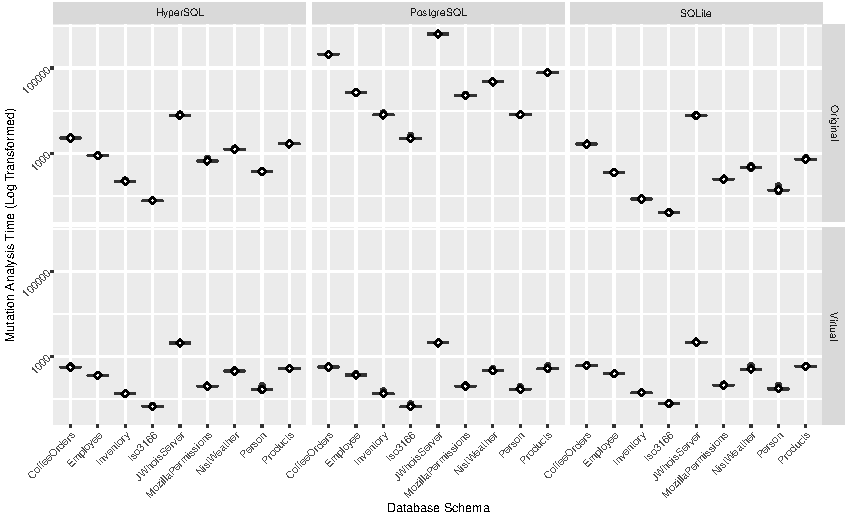
\includegraphics[scale=1.0]{graphics/graphic_bwplot_schema_analysistime_org_vm.pdf}
  \caption{Box plot of the execution time for the standard and virtual mutation analysis techniques.}
  \label{fig:graphic_bwplot_schema_analysistime_org_vm}

  % Details about the box plot from the R documentation:

  % The lower and upper "hinges" correspond to the first and third quartiles (the 25th and 75th percentiles). This differs
  % slightly from the method used by the boxplot function, and may be apparent with small samples. See boxplot.stats for for
  % more information on how hinge positions are calculated for boxplot.

  % The upper whisker extends from the hinge to the highest value that is within 1.5 * IQR of the hinge, where IQR is the
  % inter-quartile range, or distance between the first and third quartiles. The lower whisker extends from the hinge to
  % the lowest value within 1.5 * IQR of the hinge. Data beyond the end of the whiskers are outliers and plotted as points
  % (as specified by Tukey).

  {\small \justifying{ \noindent For a detailed description of the meaning of the boxes in this plot, please refer to
      Section~\ref{sec:experimental-setup}. The boxes in this plot are noticeably compressed because there is little variability in
      the timings across the different configurations.  Since the results from running the standard method on the
      \Postgres~DBMS differ substantially from those with the other techniques and databases, all of the
      data values were log-transformed, thereby best revealing the relevant trends.} \par}

  \vspace*{-1em}

\end{figure*}


Once predicates have been obtained for all integrity constraints pertaining to a database table\footnote{{\scriptsize See McMinn \etal~\cite{McMinn2015} for a full list of functions for obtaining predicates for integrity constraints used by the schemas and DBMSs that we study in this paper.}}, an {\it acceptance predicate} can be formed. An acceptance predicate describes whether a row of data (such as that which forms part of an \INSERT statement in a test case) conforms to all of the integrity constraints defined on a table, and as such, whether that row of data will be admitted into the database. An acceptance predicate is formed by the conjunction of each of the individual integrity constraint predicates.

% further examples ?

% GMK NOTE: This paragraph previously included the use of the word "we" when it was actually referencing a technique!

\inlineheading{Performing \VMA} Once acceptance predicates have been obtained for each of the tables of a database schema, they can be used to perform virtual mutation analysis. Rather than submitting the rows of data in the \INSERT~statements of a test case directly to the DBMS, rows of data can instead be evaluated by the acceptance predicate relevant to the table that is the subject of the \INSERT. With standard mutation analysis, monitoring focuses on the differences in the acceptance and rejection behavior of the DBMS with respect to the \INSERT~statements submitted as part of each test case. With \vma, however, the monitoring instead considers the difference in truth values of acceptance predicates when evaluated with the data contained within an individual \INSERT~statement. A difference in truth value of an acceptance predicate with the original schema compared to a mutant indicates that the mutant is killed by the test suite.

%% Obvious?
%As with standard mutation analysis, the virtual method can compute a mutation score.

%% PSM - no need to explain this again -- it's introduced in the background
%; that is, the number of mutants killed divided by all mutants under consideration.

% GMK NOTE: Stressing that a test suite has a minimal number of INSERTS and then revising the remaining content.

It is worth noting that mutation analysis of schemas involves the repeated execution of tests normally containing a minimal number of \INSERTs. Yet, even when running these tests, virtual mutation analysis always avoids the need to communicate with an instance of a DBMS that hosts the mutant databases. This saves the cost of setting up the tables of each database for the original schema and each of the subsequent mutants (through SQL \sql{CREATE} \sql{TABLE}s), executing the \INSERT statements in the test suite against the database, and then, finally, restoring the state of the DBMS by removing the database tables (through SQL \sql{DROP} \sql{TABLE} statements).

One disadvantage of \vma is that a model of the operation of the integrity constraints is needed for the DBMS with which we wish to test schemas and perform mutation analysis. While integrity constraints tend to operate in broadly the same way across most DBMSs there is the potential for subtle variations due to differing interpretations of the SQL standard (as shown with the primary key example with \SQLite). So, while we have models that are accurate for \HyperSQL, \Postgres and \SQLite, which we use in this paper, new models may be required for \mbox{other DBMSs}.

\inlineheading{Related Work} Although this paper is the first to present the idea of virtual mutation, there is a lot of prior work focused on improving the efficiency of mutation analysis; due to space constraints we briefly survey some of the most related approaches. For instance, Just \etal~introduced a compiler-integrated method to make mutation testing faster~\cite{Just2011}. Also, Tokumoto \etal~showed how various techniques, such as the use of virtual machines, can improve the efficiency of mutation testing~\cite{Tokumoto2016}. Finally, Tuya \etal~applied selective mutation to the mutation testing of SQL \SELECTs~\cite{Tuya2007}.



%!TEX root=../ast2016.tex

\vspace{-.5em}

\section{Experimental Setup}
\label{sec:experimental-setup}

% PURPOSE: Give the lead in to the research questions and then formally state each question

To experimentally evaluate the presented \vma technique, we investigate three research questions, comparing it against
the \Original approach to mutation analysis for relational database schemas, which uses an actual instance of a DBMS
(and is hereafter simply referred to as the ``\Original'' method).

% PSM changed the colon to a full stop because the next part currently starts on a new column and it looked odd

\vspace{5pt}

\noindent
\textbf{RQ1 (Efficiency):} How does the time overhead of \vma compare to the \Standard technique's cost, and how does
this vary depending on the DBMS in use?

\vspace{5pt}

\noindent
\textbf{RQ2 (Time Savings):} How do the time savings from using \vma vary when increasing either the number
of analysed mutants or the number of executed tests?

\vspace{5pt}

\noindent
\textbf{RQ3 (Effectiveness):} How does the mutation score of \vma compare to the score of a time-constrained \Original method that
is only permitted to run for as long as the virtual one?

% PURPOSE: Explain the number of trials and the basics about test data generation and describe the subject schemas,
% making sure to briefly mention that the chosen DBMSs are representative in nature (could not fit more content)

% {Schema} & \HyperSQL & \Postgres & \SQLite \\
% JWhoisServer & 178 & 178 & 184\\

\begin{sloppypar}
\inlineheading{Methodology} To answer the first and second research \mbox{questions}, we recorded the time needed to run the \Original approach and \vma 30 times each, for each of the subject schemas listed in Table~\ref{tbl:study-schemas} and with each of the three representative DBMSs --- \HyperSQL, \Postgres and \SQLite.  Two schemas we used appear in open-source projects (i.e., JWhoisServer and MozillaPermissions), while others appear in SQL conformance suites and DBMS sample sets (i.e., NistWeather and Iso3166, respectively). Previous studies have shown that the remaining schemas were challenging to handle for random test generators \cite{McMinn2015} and the open-source DBMonster tool \cite{Kapfhammer2013}.  Between $9$ and $184$ mutants were generated for each schema and between $426$ and $449$ in total for the three DBMSs. These totals correspond to numbers following the removal of certain ineffective mutants --- mutants found to be equivalent to the original or some other mutant, or ``stillborn'' \cite{Wright2014}. Due to differing interpretations of the SQL standard, the notion of ``equivalence'' differs from DBMS to DBMS, leading to a different number of mutants for some of the schemas (e.g., JWhoisServer yields $178$ for \HyperSQL and \Postgres and $184$ for \SQLite).
\end{sloppypar}

% PURPOSE: Give more details about the test data generation procedure

For each run, we used a test suite that was automatically generated by a search-based method with a unique random seed.  Details of the specific generation algorithms used are given by McMinn \etal~\cite{McMinn2015}. We used the alternating variable method, or \AVM, since past experiments have shown it to be the most reliable automated method for generating test suites that achieve high levels of test coverage~\cite{McMinn2015}. The coverage criterion we used was a combination of ``ClauseAICC'', ``AUCC'' and ``ANCC'', thus merging the strongest criteria for testing the integrity constraints of schemas.

% PURPOSE: Explain the third research question's process

To answer the third research question, we ran the \Original technique $30$ times, performing a mutation analysis that randomly selected mutants until the time taken for the corresponding run of the $30$ repetitions of \vma was exhausted. 
%
%% PSM: TODO-FOR-GREG I'm not sure we need this sentence. Also it is technically untrue, it's actually the minimum allotted time, although that reads a bit weird. It's minimum because it keeps selecting mutants until after the equivalent VMA time is exhausted, not before. They're never exactly equal, apart from in the cases where it's fluke....
In other words, the \Original method was run in a ``time-constrained'' fashion where its maximum allotted time was equal to the time needed to complete the comparable \vma.

% PURPOSE: State the execution environment and the tools used for the experiments

We implemented our virtual model into our \SA tool \cite{Kapfhammer2013,McMinn2015,Wright2014}, which we also used to
perform all of the experiments. \SA was compiled with the JDK 7 compiler and executed with the Linux version of the 64-bit Oracle Java 1.7 virtual machine.  Experiments were executed on an Ubuntu 14.04 workstation, with a 3.13.0-44 Linux 64-bit kernel, a quad-core 2.4GHz CPU and 12GB RAM. All input (i.e., the database schemas) and output (i.e., the result files) were stored on the workstation's local disk. We used the default configuration of \PostgreSQL version 9.3.5, \HyperSQL version 2.2.8 and \SQLite 3.8.2.  \HyperSQL and \SQLite were used with ``in-memory'' mode enabled.

% PURPOSE: Describe the meaning of the box and whisker plots

\inlineheading{Analysis Methods} Figures~\ref{fig:graphic_bwplot_schema_analysistime_org_vm} and ~\ref{fig:graphic_bwplot_schema_mutationscore_vm_tcm} furnish box and \mbox{whisker plots}.  In these plots the box itself represents the interquartile range (IQR), or the measure of statistical dispersion that is the difference between the first and third quartiles. Moreover, the upper whisker extends from the top of the box to the highest value that is within $1.5$ times the IQR, the lower whisker goes from the bottom of the box to the lowest value within $1.5$ times the IQR, and the thick horizontal line represents the median value. Also, these box plots use a filled circle for an outlier and an open diamond for the mean value.

% PURPOSE: Describe the statistical and effect size tests

\begin{sloppypar}
To statistically analyse the trends in Figure~\ref{fig:graphic_bwplot_schema_analysistime_org_vm} we conducted tests for significance with the nonparametric \wilcoxon, using the sets of 30 execution times obtained with a specific DBMS and the \Original and \vma techniques.  A \mbox{\pvalue} less than $0.05$ is deemed significant.  To complement significance tests, the nonparametric \^{A}\textsubscript{12} statistic of Vargha and Delaney \cite{Vargha2000} was used to compute effect sizes, which determine the average probability that one approach ``outperforms'' another.  We followed the guidelines of Vargha and Delaney in that an effect size is deemed to be ``large'' if the value of \atwelve~is $< 0.29$ or $> 0.71$, ``medium'' if \atwelve~is $< 0.36$ or $> 0.64$ and ``small'' if \atwelve~is $< 0.44$ or $> 0.56$.  Values of \atwelve~close to the $0.5$ value are viewed as showing no effect.  When discussing effect sizes for the execution times of the two methods, we follow Neumann \etal~\cite{Neumann2015} and say that a value of \atwelve closer to zero indicates that virtual is the preferred technique while a value near one shows that \Original is faster.
\end{sloppypar}

% PURPOSE: Describe the calculation of the percentage of mean time saved

As the number of mutants subject to analysis and the number of generated tests increases, Figure~\ref{fig:graphic_scatterplot_mutantstests_percentagetimesaved} plots the percentage of mean time saved from using \vma instead of the \Original method.  This value is determined by first calculating the mean execution time from the $30$ trials of both the \Standard and the \virtual techniques. If $T_s$ denotes the mean time taken by the standard method and $T_v$ is the mean time needed for the virtual one, then we calculated the percentage of mean time saved by $({T_s - T_v})/{T_s}$.

% PURPOSE: Describe the calculation of the correlation coefficient

We employed a correlation statistic to determine how the mutation scores of the \tc method correspond to those of \vma.  Due to the possibility of rank ties, which are not supported by a number of correlation measures, we chose to use the tie-aware Kendall's \taub~coefficient, as provided by the ``Kendall'' R package \cite{KendallCran}.  Kendall's \taub~provides a measurement of correlation between -1 and 1, representing a strong negative and strong positive association, respectively, with 0 indicating that there is no correlation. Following Inozemtseva and Holmes, we adopt the Guildford scale to describe the correlation values, with the absolute value of a coefficient being described as ``low'' when it is less than $0.4$, ``moderate'' when it is between $0.4$ and $0.7$, ``high'' when ranging from $0.7$ to $0.9$, and ``very high'' when it is greater than \mbox{$0.9$ \cite{Inozemtseva2014}}.

% GRAPHIC: This is the figure that will contain the graphs for the percentage and the number of mutants (and tests)
% NOTE: This input had to be moved to this location in the code to ensure that the graphs were properly spaced.
% SCATTERPLOT INPUT
%!TEX root=ast2016.tex

\begin{figure*}[t]
  \centering
  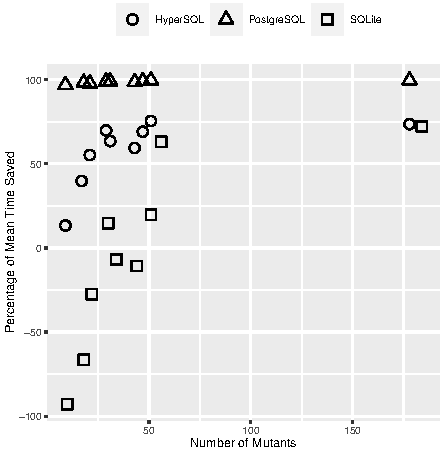
\includegraphics[scale=1.0]{graphics/graphic_scatterplot_nummutants_percentage.pdf}
  \caption{Box plot of the execution time for the original and virtual mutation analysis techniques.}
  \label{fig:graphic_bwplot_schema_analysistime_org_vm}

  % Details about the box plot from the R documentation:

  % The lower and upper "hinges" correspond to the first and third quartiles (the 25th and 75th percentiles). This differs
  % slightly from the method used by the boxplot function, and may be apparent with small samples. See boxplot.stats for for
  % more information on how hinge positions are calculated for boxplot.

  % The upper whisker extends from the hinge to the highest value that is within 1.5 * IQR of the hinge, where IQR is the
  % inter-quartile range, or distance between the first and third quartiles. The lower whisker extends from the hinge to
  % the lowest value within 1.5 * IQR of the hinge. Data beyond the end of the whiskers are outliers and plotted as points
  % (as specified by Tukey).

  % Commentary on the results in this output:

  % - Note that this data has been "log transformed" using a log-to-the-base-ten transformation
  % - Transformation is done because the Postgres-Original data is on a different scale than all other data
  % - This means that you will only see variation for Postgres-Original (without transformation)
  % - Using the log-transformed data shows the basic trends in the data sets

  {\small \justifying{ \noindent In this plot the box itself represents the interquartile range (IQR), or the measure of
      statistical dispersion that is the difference between the first and third quartiles. Furthermore, the upper
      whisker extends from the top of the box to the highest value that is within 1.5 times the IQR, the lower whisker
      goes from the bottom of the box to the lowest value within 1.5 times the IQR, and the thick horizontal line
      represents the median value. The boxes in this plot are noticeably compressed because there is little variance in
      the timings across the different configurations.  Since the results from running the original method on the
      \Postgres DBMS differ substantially from those with the other techniques and databases, all of the
      data values were log-transformed, thereby best revealing the relevant trends.} \par}

\end{figure*}


% GRAPHIC: This is the box and whisker plot that shows the mutation score for the two techniques
% BOXPLOT input
%!TEX root=ast2016.tex

\begin{figure*}[t]
  \centering
  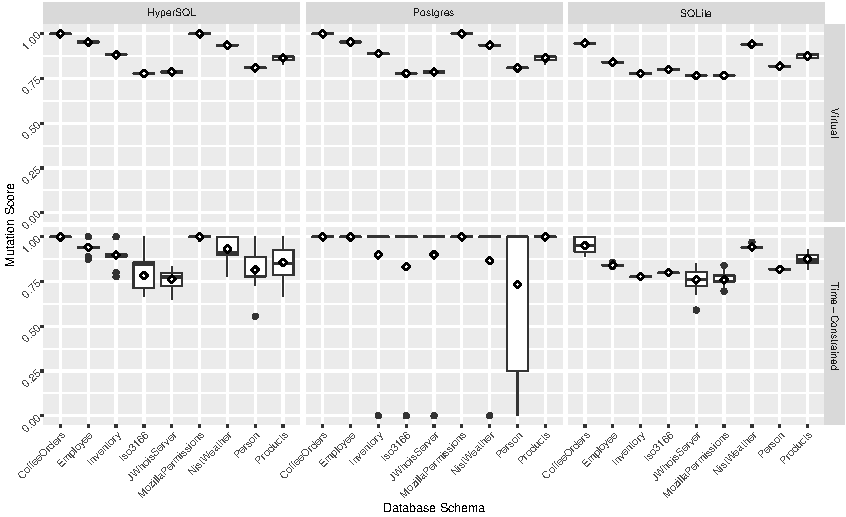
\includegraphics[scale=1.0]{graphics/graphic_bwplot_schema_mutationscore_vm_tcm.pdf}
  \caption{Box plot of the mutation score for the virtual and time-constrained mutation analysis techniques.}\label{fig:graphic_bwplot_schema_mutationscore_vm_tcm}

  % NOTE: This caption is not yet correct.

  {\small \justifying{\noindent The meaning for this box plot's elements is the same as the meaning of those described
      in the subcaption of Figure~\ref{fig:graphic_bwplot_schema_analysistime_org_vm}. Additionally, in this box plot a
      filled circle denotes an outlier and the open diamond is the mean value. Using test suites from thirty separate
      runs of the search-based test data generation method developed by McMinn \etal~\cite{McMinn2015}, this plot shows
      the variation in the mutation score for both the virtual and the time-constrained method and for all of the chosen
  relational schemas and the three database management systems. } \par}

\end{figure*}


% These are the threats to validity:

% -- Randomness in the SA tool and the generated test suite
% -- Randomness in the selection of mutants for time-constrained
% -- Variability in the running time of the mutation analysis
% ---> So, ran multiple trials and did statistical analysis
% ---> When calculated effect sizes, we also looked at thresholds

\inlineheading{Threats to Validity} There are several threats to the validity of the empirical results presented in this paper. First, several of the techniques that we used (e.g., the test data generator in \SA and the mutant selection by the \tcm~method) employ randomness. Additionally, background processes running during experimentation may introduce small random differences in the timings for the mutation analysis methods. To control for these threats we ran 30 trials and used box and whisker plots and statistical tests to analyse the results. Adhering to the advice of Neumann \etal~\cite{Neumann2015}, we disregarded all timings below $100$ ms --- as they would not be perceived by users of our tool --- to ensure that we did not misapply the Vargha-Delaney \mbox{effect size}.

% -- Defects in the test data generator
% -- Defects in the virtual mutation analysis
% ---> So, we tested these programs and checked the mutation scores

% -- Defects in the analysis routines
% --> So, we tested this these programs

Another threat to the validity of our results is defects in the test data generator or one of the mutation analysis techniques. We controlled these threats by implementing and regularly applying an automated test suite for all of these software tools; to ensure their correct operation we also manually performed ``spot checks'' on small schemas. In addition, we verified that the \vma always yielded the same mutation score as the \Original one. Finally, since defects in our analysis routines would compromise the conclusions from our experiments, we created and regularly ran tests for the R code that manipulated the data, performed statistical tests and effect size computations, and visualised the results.

% -- Limited number of subjects in the empirical study
% --> But, these subjects are "representative" and open-source

While the rich and diverse nature of real software systems makes it impossible for us to claim that our schemas are representative of all the characteristics of all possible relational database schemas, we endeavored to select schemas from a wide variety of sources, comprising open-source programs, conformance suites for the SQL standard and schemas from databases that were used in previous studies. Table~\ref{tbl:study-schemas} shows the variety captured by the schemas, with tables that contain 1--50 constraints, including \CHECKs, \FKs, \PKs, \NOTNULLs and \UNIQUEs.

%!TEX root=ast2016.tex

% \section{Empirical Study}
% \label{sec:empirical-study}

\section{Experimental Setup}
\label{sec:experimental-setup}

% TODO: Add in one introductory sentence to start off this section

\subsection{Relational Database Schemas}
\label{sec:subjects}

%!TEX root=../ast2016.tex

\begin{table}[t!]
	\caption{Schemas analysed in the empirical study} \label{tbl:study-schemas}
	\scriptsize
	\centering
	\scalebox{\tablescalefactor}{
		\begin{tabular}{l@{\hskip -5pt}rrrrrrrr}
			{Schema}           & \rot{Tables} & \rot{Columns} & \rot{Checks} & \rot{Foreign Keys} & \rot{Not Nulls} & \rot{Primary Keys} & \rot{Uniques} & \rot{$\sum$Constraints} \\ \hline
			ArtistSimilarity & 2 & 3 & 0 & 2 & 0 & 1 & 0 & 3 \\
			ArtistTerm & 5 & 7 & 0 & 4 & 0 & 3 & 0 & 7 \\
			BankAccount & 2 & 9 & 0 & 1 & 5 & 2 & 0 & 8 \\
			BookTown & 22 & 67 & 2 & 0 & 15 & 11 & 0 & 28 \\
			BrowserCookies & 2 & 13 & 2 & 1 & 4 & 2 & 1 & 10 \\
			Cloc & 2 & 10 & 0 & 0 & 0 & 0 & 0 & 0 \\
			CoffeeOrders & 5 & 20 & 0 & 4 & 10 & 5 & 0 & 19 \\
			CustomerOrder & 7 & 32 & 1 & 7 & 27 & 7 & 0 & 42 \\
			DellStore & 8 & 52 & 0 & 0 & 39 & 0 & 0 & 39 \\
			Employee & 1 & 7 & 3 & 0 & 0 & 1 & 0 & 4 \\
			Examination & 2 & 21 & 6 & 1 & 0 & 2 & 0 & 9 \\
			Flights & 2 & 13 & 1 & 1 & 6 & 2 & 0 & 10 \\
			FrenchTowns & 3 & 14 & 0 & 2 & 13 & 0 & 9 & 24 \\
			Inventory & 1 & 4 & 0 & 0 & 0 & 1 & 1 & 2 \\
			Iso3166 & 1 & 3 & 0 & 0 & 2 & 1 & 0 & 3 \\
			iTrust & 42 & 309 & 8 & 1 & 88 & 37 & 0 & 134 \\
			JWhoisServer & 6 & 49 & 0 & 0 & 44 & 6 & 0 & 50 \\
			MozillaExtensions & 6 & 51 & 0 & 0 & 0 & 2 & 5 & 7 \\
			MozillaPermissions & 1 & 8 & 0 & 0 & 0 & 1 & 0 & 1 \\
			NistDML181 & 2 & 7 & 0 & 1 & 0 & 1 & 0 & 2 \\
			NistDML182 & 2 & 32 & 0 & 1 & 0 & 1 & 0 & 2 \\
			NistDML183 & 2 & 6 & 0 & 1 & 0 & 0 & 1 & 2 \\
			NistWeather & 2 & 9 & 5 & 1 & 5 & 2 & 0 & 13 \\
			NistXTS748 & 1 & 3 & 1 & 0 & 1 & 0 & 1 & 3 \\
			NistXTS749 & 2 & 7 & 1 & 1 & 3 & 2 & 0 & 7 \\
			Person & 1 & 5 & 1 & 0 & 5 & 1 & 0 & 7 \\
			Products & 3 & 9 & 4 & 2 & 5 & 3 & 0 & 14 \\
			RiskIt & 13 & 57 & 0 & 10 & 15 & 11 & 0 & 36 \\
			StackOverflow & 4 & 43 & 0 & 0 & 5 & 0 & 0 & 5 \\
			StudentResidence & 2 & 6 & 3 & 1 & 2 & 2 & 0 & 8 \\
			UnixUsage & 8 & 32 & 0 & 7 & 10 & 7 & 0 & 24 \\
			Usda & 10 & 67 & 0 & 0 & 31 & 0 & 0 & 31 \\
			\hline
			{Total} & 172 & 975 & 38 & 49 & 335 & 114 & 18 & 554 \\
			\hline

		\end{tabular}
	}
\end{table}


\begin{itemize}
  \item 32 schemas
    \begin{itemize}
      \item 1 to 42 tables
      \item 3 to 309 columns
      \item 0 to 134 constraints
      \item Includes each of the types of constraint supported by \SchemaAnalyst (\PK, \FK, \NOTNULL, \UNIQUE and \CHECK constraints)
    \end{itemize}
  \item 3 DBMSs -- \Postgres, \HyperSQL (in-memory), \SQLite (in-memory)
  \item 30 repeated trials
  \item 2 techniques -- \Original and \VirtualMutationAnalysis
  \item Metrics -- time taken for mutation analysis, number of mutants, number of test cases
  \item Mention that the mutation scores of the Original technique are used to validate the results given by virtual mutation analysis, and that in every case the results were identical. (Possibly repeat this in the threats section?)
\end{itemize}

\subsection{Research Questions}
\label{sec:research-questions}

The experiments in this paper investigate three research questions, which we state in the following fashion.

\vspace{5pt}

\noindent
\textbf{RQ1 (Efficiency):} How does the time overhead of \vma compare to the \Standard technique's cost, and how does
this vary depending on the DBMS in use?

\vspace{5pt}

\noindent
\textbf{RQ2 (Scalability):} How does the time savings from using \vma scale when increasing either the number
of analysed mutants or the number of executed tests?

\vspace{5pt}

\noindent
\textbf{RQ3 (Effectiveness):} How does the mutation score of \vma compare to the score of a time-constrained method that
is only permitted to run for as long as the virtual one?

\subsection{Methodology}
\label{sec:methodology}

% Explain the number of trials and the basics about test data generation

To answer the first and second research questions, we ran the \Original technique and \vma 30 times each, for every one of the schemas in Table~\ref{tbl:study-schemas} and with each of the three DBMSs, recording the time taken. For each run, we used a test suite that was automatically generated by a search-based method; the test generator was seeded with a unique random value.

% Give more details about the test data generation procedure

Details of the specific test suite generation algorithms used are given by McMinn \etal~\cite{McMinn2015}. We used the \AVM technique since past experiments have show it to be the most reliable automated method for generating test suites that achieve high levels of test coverage~\cite{McMinn2015}. The coverage criterion we used was a combination of ``ClauseAICC'', ``AUCC'' and ``ANCC'', thus merging the strongest criteria for testing the integrity constraints of database schemas.

% Explain the third research question's process

To answer the third research question, we ran the \Original technique 30 times, performing a mutation analysis that randomly selected mutants until the time taken for the corresponding run of the 30 repetitions of \vma was exhausted. In other words, the \Original method was run in a ``time-constrained'' fashion where its maximum allotted time was equal to the time needed to complete the comparable \vma.

% State the execution environment and the tools used for the experiments

We performed all of the experiments with the \SA tool \cite{Kapfhammer2013,McMinn2015,Wright2014}, compiled with the Java Development Kit 7 compiler and executed with the Linux version of the 64-bit Oracle Java 1.7 virtual machine.  Experiments were executed on an Ubuntu 14.04 workstation, with a 3.13.0-44 Linux 64-bit kernel, a quad-core 2.4GHz CPU and 12GB RAM. All input (i.e., the database schemas) and output (i.e., the result files) were stored on the workstation's local disk. We used the default configuration of \PostgreSQL version 9.3.5, \HyperSQL version 2.2.8 and \SQLite 3.8.2.  \HyperSQL and \SQLite were used with ``in-memory'' mode enabled.

\subsection{Analysis Methods}
\label{sec:analysis-methods}

% Describe the meaning of the box and whisker plots

Figures~\ref{fig:graphic_bwplot_schema_analysistime_org_vm} and ~\ref{fig:graphic_bwplot_schema_mutationscore_vm_tcm} furnish box and whisker plots.  In these plots the box itself represents the interquartile range (IQR), or the measure of statistical dispersion that is the difference between the first and third quartiles. Moreover, the upper whisker extends from the top of the box to the highest value that is within $1.5$ times the IQR, the lower whisker goes from the bottom of the box to the lowest value within $1.5$ times the IQR, and the thick horizontal line represents the median value.  Additionally, these box plots use a filled circle for an outlier and an open diamond for the mean value.

% Describe the statistical and effect size tests

To statistically analyse the trends in Figure~\ref{fig:graphic_bwplot_schema_analysistime_org_vm} we conducted tests for significance with the nonparametric Wilcoxon rank-sum test, using the sets of 30 execution times obtained with a specific DBMS and the \Original and \vma techniques.  A {\it p}-value less than $0.05$ is deemed to be significant.  To complement significance tests, the nonparametric \^{A}\textsubscript{12} statistic of Vargha and Delaney \cite{Vargha2000} was used to compute effect sizes, which determine the average probability that one approach ``out performs'' another.  We followed the guidelines of Vargha and Delaney in that an effect size is deemed to be ``large'' if the value of \atwelve~is $< 0.29$ or $> 0.71$, ``medium'' if \atwelve~is $< 0.36$ or $> 0.64$ and ``small'' if \atwelve~is $< 0.44$ or $> 0.56$.  Values of \atwelve~close to the $0.5$ value are deemed to have no effect size.  When discussing effect sizes for the execution times of the two methods, we follow Neumann \etal~\cite{Neumann2015} and say that a value of \atwelve closer to zero indicates that virtual is the preferred technique while a value near one shows that \Original is faster.

% Describe the calculation of the percentage of mean time saved and the correlation coefficient

\subsection{Threats to Validity}
\label{sec:threats-to-validity}

% TODO: Explain that we check the mutation score to ensure that Standard and Virtual are the same!
% TODO: Reference the SSBSE 2015 paper that talks about transformation of the values; we also
% did this and we are certain that there is no difference (we also looked at different thresholds).

\section{Empirical Results}
\label{sec:empirical-results}

% PURPOSE: Compare the virtual mutation technique to the original one in terms of their execution time, showing that
% virtual mutation is often significantly faster than the standard approach to mutation analysis.

\subsection{Comparing Original and Virtual Mutation}
\label{sec:empirical-study-RQ-original-virtual-time}
% vim: ft=tex
%!TEX root=ast2016.tex

% PURPOSE: Discuss the trends in the first graph, sketching at a high level

\inlineheading{Comparing Standard and Virtual Mutation}~The box and whisker plots in Figure~\ref{fig:graphic_bwplot_schema_analysistime_org_vm} show the mutation analysis time for the two techniques across all of the relational schemas and the three DBMSs. This plot reveals that, when using the \HyperSQL~DBMS, the \virtual~method is faster than the \Original~one, especially for large schemas such as JWhoisServer. Since \Postgres~is a ``heavyweight'' disk-based DBMS, \vma~demonstrates much lower execution times than the \Original~method because it avoids database interactions. Yet, these plots show that the performance of the virtual approach is similar to the standard one when mutation analysis runs on the high-performance \sqlite~DBMS.

% PURPOSE: Analyse the trends further through the statistical analysis and the effect size computations. For effect
% sizes, make sure to comment on the fact that we did thresholding of the scores.

The statistical tests and effect size calculations confirm the trends evident in Figure~\ref{fig:graphic_bwplot_schema_analysistime_org_vm}. When comparing the timings for the two mutation analysis methods on the \HyperSQL~and \Postgres~DBMSs, the \wilcoxon~reveals, with a \pvalue~near zero, that virtual is faster than \Original~in a statistically significant fashion. Moreover, the \atwelve~values of $0.26$ and $0.0008$ for the timings on \HyperSQL~and \Postgres, respectively, show that there is a large effect size evident in the timings and thus sustain \vma~as the clear winner for efficiency. Returning a \pvalue~of $0.905$, the \wilcoxon~confirms that there is no statistical difference between the standard and virtual methods when mutation runs on \sqlite. An effect size of $0.503$, indicating that the two techniques are stochastically equivalent, further shows that a fast DBMS obviates the benefits of virtual mutation.\footnote{{\scriptsize Following the suggestions of Neumann \etal~\cite{Neumann2015}, we also transformed the effect size values by discarding all timings below $100$ milliseconds, ultimately yielding the same conclusions as reported for the untransformed data values.}}



% PURPOSE: Investigate the scalability of virtual mutation, looking at how the percentage of mean time saved varies as
% the number of mutants and the number of tests increases, revealing the best configurations for this method.

\subsection{Scalability of Virtual Mutation}
\label{sec:empirical-study-RQ-scalability-mutants-tests}
% vim: ft=tex
%!TEX root=ast2016.tex

% Here are the percentage savings values. You can also render the RMarkdown file to get results like this.

               % schema       dbms     Standard    Virtual       saving saving_percent mutantcount testcount
               %  (chr)      (chr)        (dbl)      (dbl)        (dbl)          (dbl)       (int)     (int)
% 1            Products PostgreSQL  78427.20000  516.40000  77910.80000     0.99341555          47        46
% 2            Products   HyperSQL   1667.50000  515.20000   1152.30000     0.69103448          47        46
% 3            Products     SQLite    724.40000  582.00000    142.40000     0.19657648          51        52
% 4              Person PostgreSQL   8077.50000  169.36667   7908.13333     0.97903229          21        19
% 5              Person   HyperSQL    374.13333  167.36667    206.76667     0.55265502          21        19
% 6              Person     SQLite    136.83333  174.53333    -37.70000    -0.27551766          22        20
% 7         NistWeather PostgreSQL  47717.63333  461.90000  47255.73333     0.99032014          31        52
% 8         NistWeather   HyperSQL   1238.83333  451.53333    787.30000     0.63551729          31        52
% 9         NistWeather     SQLite    471.63333  503.96667    -32.33333    -0.06855608          34        56
% 10 MozillaPermissions PostgreSQL  22871.53333  198.93333  22672.60000     0.99130214          29        32
% 11 MozillaPermissions   HyperSQL    662.13333  199.56667    462.56667     0.69860048          29        32
% 12 MozillaPermissions     SQLite    246.20000  209.96667     36.23333     0.14717032          30        33
% 13       JWhoisServer PostgreSQL 631285.63333 2088.00000 629197.63333     0.99669246         178       152
% 14       JWhoisServer   HyperSQL   7805.26667 2060.30000   5744.96667     0.73603721         178       152
% 15       JWhoisServer     SQLite   7707.66667 2139.93333   5567.73333     0.72236302         184       158
% 16            Iso3166 PostgreSQL   2225.80000   66.56667   2159.23333     0.97009315           9         9
% 17            Iso3166   HyperSQL     77.03333   66.76667     10.26667     0.13327564           9         9
% 18            Iso3166     SQLite     40.43333   78.00000    -37.56667    -0.92910140          10        12
% 19          Inventory PostgreSQL   7986.60000  133.50000   7853.10000     0.98328450          18        16
% 20          Inventory   HyperSQL    220.06667  132.43333     87.63333     0.39821266          17        16
% 21          Inventory     SQLite     84.00000  139.83333    -55.83333    -0.66468254          18        18
% 22           Employee PostgreSQL  26860.73333  367.80000  26492.93333     0.98630715          43        35
% 23           Employee   HyperSQL    881.83333  357.73333    524.10000     0.59432999          43        35
% 24           Employee     SQLite    353.26667  391.16667    -37.90000    -0.10728439          44        38
% 25       CoffeeOrders PostgreSQL 211013.40000  563.23333 210450.16667     0.99733082          51        77
% 26       CoffeeOrders   HyperSQL   2276.83333  558.40000   1718.43333     0.75474709          51        77
% 27       CoffeeOrders     SQLite   1642.26667  606.70000   1035.56667     0.63057157          56        90

% PURPOSE: Explain the results for the PostgreSQL and HyperSQL database management systems

\inlineheading{Saving Time with Virtual Mutation} As evident by the scatter plot in Figure~\ref{fig:graphic_scatterplot_mutantstests_percentagetimesaved}, it is worthwhile to see how the time savings associated with using \virtualmutationanalysis~varies as the number of mutants and tests increases. Since \postgres~is a heavyweight DBMS relative to \HyperSQL~and \sqlite, this scatter plot reveals that, by avoiding database interactions, the \virtual~method yields substantial savings regardless of the number of mutants subject to analysis of the number of tests run.  Figure~\ref{fig:graphic_scatterplot_mutantstests_percentagetimesaved} also affirms that using \virtual~mutation on \HyperSQL~saves time, albeit in a way that is gradual and tapering off as there are more mutants and tests.

% PURPOSE: Discuss how the SQLite database management system and small schemas is faster than virtual

The scatter plots also highlight the fact that, when run on \sqlite, \virtual~only improves the performance of mutation analysis for four of the nine schemas. While these larger schemas see reduced overheads with the \virtual~technique, the $5$ smaller schemas do not benefit from the decrease in database interactions afforded by the presented method --- thus leading to the negative values of the percentage of mean time saved seen in Figure~\ref{fig:graphic_scatterplot_mutantstests_percentagetimesaved}. Yet, even in cases in which a small schema and a fast DBMS should outperform \vma, we found that the difference in execution time was always less than 100 milliseconds, a negligible amount that experts agree is not perceivable by users of a software tool~\cite{Neumann2015}.




% PURPOSE: Compare the virtual and time-constrained techniques in terms of their mutation score and the number of
% mutants that are actually executed during mutation analysis, showing the superiority of virtual mutation.

\subsection{Virtual and Time-Constrained Mutation}
\label{sec:empirical-study-RQ-virtual-time-constrained-virtual}
% vim: ft=tex
%!TEX root=ast2016.tex

% GRAPHIC: This is the box and whisker plot that shows the mutation score for the two techniques
%!TEX root=ast2016.tex

\begin{figure*}[t]
  \centering
  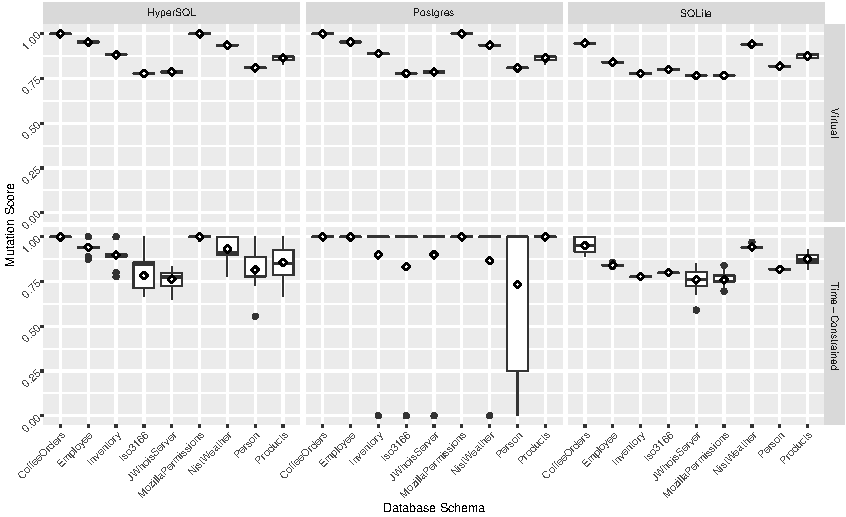
\includegraphics[scale=1.0]{graphics/graphic_bwplot_schema_mutationscore_vm_tcm.pdf}
  \caption{Box plot of the mutation score for the virtual and time-constrained mutation analysis techniques.}\label{fig:graphic_bwplot_schema_mutationscore_vm_tcm}

  % NOTE: This caption is not yet correct.

  {\small \justifying{\noindent The meaning for this box plot's elements is the same as the meaning of those described
      in the subcaption of Figure~\ref{fig:graphic_bwplot_schema_analysistime_org_vm}. Additionally, in this box plot a
      filled circle denotes an outlier and the open diamond is the mean value. Using test suites from thirty separate
      runs of the search-based test data generation method developed by McMinn \etal~\cite{McMinn2015}, this plot shows
      the variation in the mutation score for both the virtual and the time-constrained method and for all of the chosen
  relational schemas and the three database management systems. } \par}

\end{figure*}


% GRAPHIC: This is the bar chart of the number of mutants that each technique ran during mutation analysis
% NOTE: This graph was removed due to space constraints, it can be summarized in the text, I think.
% %!TEX root=ast2016.tex

\begin{figure*}[t]
  \centering
  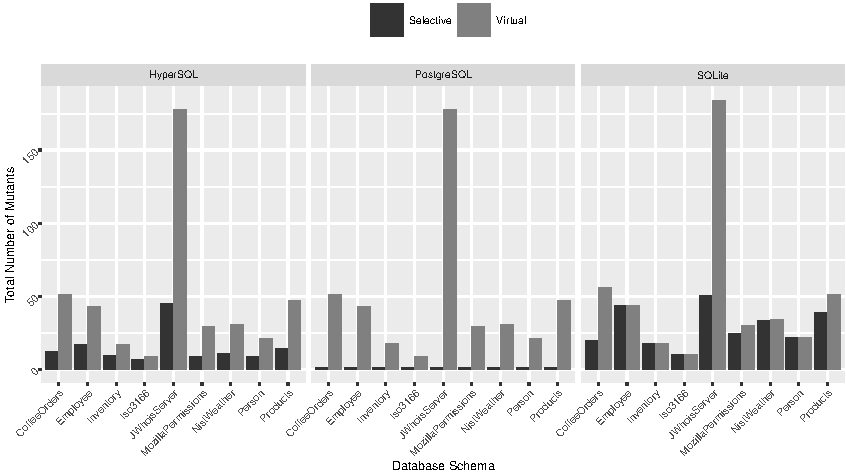
\includegraphics[scale=1.0]{graphics/graphic_barplot_schema_mutantcount_vm_tcm.pdf}
  \caption{Bar plot of the mutant count for both the virtual and time-constrained mutation analysis techniques.}
  \label{fig:graphic_barplot_schema_mutantcount_vm_tcm}

  {\small \justifying{ \noindent In this plot the height of the bar corresponds to the number of mutants subject to
      analysis by the virtual and time-constrained methods; this count is reported for all of the chosen relational
      schemas and the three database management systems. Since the time-constrained technique employs randomness to
      select mutants that can be run within a specified time limit, the height of a light grey bar is the average across
      a total of thirty runs; virtual mutation analysis is deterministic and thus the height of the dark grey bar is a
      direct count. } \par}

\end{figure*}


\inlineheading{Virtual and Time-Constrained Mutation} Since the experiments revealed that \vma~is faster than the \Original~one in $22$ out of the $27$ studied configurations --- and competitive with the DBMS-based method in the other $5$ --- it is useful to ascertain whether the presented technique might yield more accurate mutation scores in some circumstances. To this end, Figure~\ref{fig:graphic_bwplot_schema_mutationscore_vm_tcm} presents the mutation score of both the virtual approach and a time-limited analysis in which \Original~randomly analyses mutants for as long as virtual. These box plots show that the time-constrained technique results in mutation scores that are often highly variable. This result can be attributed to randomness inherent in running mutation analysis under a strict time limit that will not permit the examination of every mutant. For instance, the noticeable variability in mutation score when the Person schema is run on \Postgres~is due to the possibility of not finishing the analysis of the first mutant.

Bearing in mind that the virtual method produces mutation scores that are always equal to those achieved by the standard technique, it is also important to observe that time-constrained mutation analysis leads to overly high mutation scores.  Yet, at least for the \HyperSQL~and \SQLite~DBMSs, the box plots in Figure~\ref{fig:graphic_bwplot_schema_mutationscore_vm_tcm} suggest that the mutation scores are roughly similar for \vma~and the time-constrained method. To rigorously establish this correlation, we calculated Kendall's \taub~for the two techniques on each of the DBMSs, arriving at the values of $0.561$ (moderate), $0.132$ (low) and $0.756$ (high) for \HyperSQL, \PostgreSQL and \sqlite, respectively. These correlations suggest that virtual mutation is the best option when highly accurate scores are needed and there is limited time for mutation analysis of a database schema.

% These correlations suggest that the time-constrained mutation
% analysis of a schema for fast, in-memory databases like \HyperSQL~and \sqlite~leads to scores that respectively have a
% moderate and high correlation with the actual score. Yet, the scores produced by virtual and time-constrained mutation
% analysis on \postgres~have a low correlation. Overall, these results indicate that virtual mutation is the best option





%!TEX root=../ast2016.tex

\section{Conclusions}
\label{sec:conclusions}
In this paper, we have introduced a more cost-effective, scalable technique for performing mutation analysis for relational database schemas. Our technique, \vma, executes test suites virtually against a model of the mutated database schema. This removes the need to setup an instance of a database with the mutated schema on a real DBMS, and communicate with the DBMS over a socket connection to set the database up, execute SQL the \INSERT statements of a test case against it, and then clear the database down ready for the next test case. In an empirical evaluation of our technique, we found that .... %TODO -- summary of empirical findings


\vspace*{-.5em}

\scriptsize
\bibliographystyle{plain}
\bibliography{database}

\end{document}
